\documentclass[12pt, titlepage]{article}
\usepackage[utf8]{inputenc}
\usepackage[margin=1in]{geometry}

\title{Scholarly Report: Graduate Coursework in Computer Science}
\author{Victor Zhang}
\date{April 2022}

\usepackage[utf8]{inputenc}
\usepackage{amsmath}
\usepackage{amsfonts}
\usepackage[title]{appendix}
\usepackage[square,numbers]{natbib}
\usepackage{graphicx}
% \usepackage{changepage}
\usepackage{amssymb}
\usepackage{xfrac}
% \usepackage{bm}
% \usepackage{empheq}
\usepackage{dirtytalk} % quotation marks
\usepackage{setspace} % double space
\usepackage{fancyhdr} % running headers
\usepackage{times}
\usepackage{color}
\usepackage{hyperref}
\hypersetup{
    colorlinks=true, %set true if you want colored links
    linktoc=all,     %set to all if you want both sections and subsections linked
    linkcolor=blue,  %choose some color if you want links to stand out
}
\usepackage{subcaption}
\usepackage{url}
\usepackage{booktabs} % top/bottom rules
% \usepackage{cleveref}
\bibliographystyle{abbrvnat}

\newcommand{\contra}{\raisebox{\depth}{\#}}

\newenvironment{myindentpar}[1]
  {\begin{list}{}
          {
            \setlength{\leftmargin}{#1}
            \setlength{\rightmargin}{#1}
          }
          \item[]
  }
  {\end{list}}

\pagestyle{fancy}
\lhead{Graduate Coursework in Computer Science}
\rhead{Zhang}
\doublespace

\begin{document}

\maketitle
% \begin{center}
% {\huge Econ 482 \hspace{0.5cm} HW 3}\
% {\Large \textbf{Victor Zhang}}\
% {\Large February 18, 2020}
% \end{center}
\tableofcontents
\newpage

\section{Introduction}
What does it mean for a computer to be intelligent? With all the buzz around artificial intelligence and machine learning, there seems to be no end to what we can get computers to do. From automatic subtitling of youtube videos to predicting traffic times, AI and ML have made our lives infinitely easier---and the companies that develop them incredibly rich. There is no limit to what we can do with AI, or so we're told. And yet progress is painfully slow. Tesla has promised self-driving cars for over half a decade; but even the newest line of \say{autopilot} is little more than a glorified radio transmitter that can keep your car in your lane, but only on highways and in good weather. So how come years of development and thousands of the brightest minds in computer science have managed to perform as well as the worst human driver? This was the question that inspired me to study artificial intelligence. Why are machines so good at doing inhuman feats of calculation yet suck so much at basic life tasks?

The term \textit{artificial intelligence} was coined in the early days of AI research when we were optimistic about our progress and adoption of technology. From the Latin \textit{artificium}, meaning \say{a craft; a making by art}, \textit{artifice} is a broad synonym for creativity and creation. Thus, artificial intelligence is by definition intelligence created through ingenuity---human ingenuity.

Indeed, it seems the human is the perfect learning machine. From birth, we are constantly learning: movement, language, object identification, tool use. Getting an AI to learn even one of these is a monumental task, even with today's technology. And we do it all at the same time with still-underdeveloped brains. As such, humans serve as the only example of so-called \textit{general intelligence} in existence. AI researchers quickly gave up trying to build general intelligences as far too intractable. But what about learning one task at a time? For instance, learning to identify faces in pictures or footpaths from a satellite image. This has proved far more tractable for AI models and thus served as a jumping-off point for my study.

\section{Curiosity}
As a computer scientist, the first step to solving a problem is to figure out how you yourself would solve the problem. For instance, if your task was to complete a sudoku, you might consider trying each number one by one until you find a combination that works. Once you have a theoretical solution, you can then implement that using code and formal logic. These problems are thus \say{easy} for computers to solve. Even the hardest of sudokus can be solved by simply following an intuitive, understanable procedure. Now think about how you would identify a face. Well, you could say a face has to has two eyes, a nose, and a mouth. But then if you see a picture of a person wearing a mask, you can still tell it as a face, even though you can't see their nose or mouth. And things like electrical outlets seem to check all the boxes yet are clearly not faces. Suddenly, things get a lot tougher, right?

This thought experiment is mostly for illustration, since this problem has essentially been solved already by the folks at Google. Fortunately, the researchers working on this have published their work.
\begin{myindentpar}{1em}
FaceNet uses a deep convolutional network\ldots Our network consists of a batch input layer and a deep CNN followed by $L_2$ normalization, which results in the face embedding. This is followed by the triplet loss during training \cite{SchroffKP15}.
\end{myindentpar}
Woah. This doesn't seem intuitive at all! What's a convolutional network? Why is it deep? And what's normalization? As I learned more and more about the state-of-the-art in machine learning, the more questions I had.

The field as a whole has been dominated almost completely by these \textit{artificial neural networks} and their application, \textit{deep learning}. If you want to publish new results today, it is an unspoken requirement that you use a deep neural net. But why, I wondered. What about deep learning made it so good at these previously intractable tasks and what was its limitations? And what about models that didn't involve these weird neuron thingies? One model that captured my interest was \textit{hidden Markov models}. These are mathematical models derived from \textit{Markov chains}, a type of probabilistic evolution model. Having studied Markov chains in my probability classes, I was intruiged by what they could contribute in this neural net-dominated field. To satisfy my curiosity, I took two graduate classes: Principles of AI, an overview of the history and guiding principles that have shaped the development of AI systems; and Machine Learning, a class that focused on work in the last decade, i.e. neural nets. It was my goal with these two classes to understand the field holistically, from its inception to today.


\section{Knowledge}
In this section, I will present two projects I worked on as part of the two graduate classes I took. The first is a Markov-based genre classifier for long-form text. The second is a deep learning model that infers ingredients and cooking instructions from a picture of food. The first project I completed as part of the evaluation for Principles of AI, the second for Machine Learning. The first project was an unstructured research project so I will present the entire research process, from hypothesis to conclusions and future work. The second was structured by the professor, so I will outline my work and discuss my scholarly experience in the conclusion section.

% -----------------------------------------------------------------------------
% ---------------------------------GENRE DISCRIMINATION------------------------
% -----------------------------------------------------------------------------
\section{Textual Genre Discrimination using Dynamic Syntactic Features}
\subsection{Introduction}
Textual genre discrimination is an important preprocessing task for many industrial and research applications, including classification, retrieval, and higher-order NLP tasks \cite{LeeMyaeng}. The bulk of the current literature has focused on offline methods, that is, using only the text and insights gathered from the text to perform classification. Even still, the state of the art achieves an accuracy rate of around 92\% \cite{SoA}. Many classification schemes focus on low-level textual features (sentence length, word length) or lexical features (occurrence rate of common words, noun-to-verb ratio)\cite{KitchSink}. Very little analysis has been done on syntactic features. These features include depth of sentence parse trees, arity of verbal predicates, or dependency link lengths \cite{Italian}. Whereas these are the highest-level features explored by AI efforts, these are usually the lowest-level features considered by humans making the same classifications. I thus postulated that syntactic features represent a wealth of untapped potential for accurate classification schemes.

In this project I focused my attention on \textit{part of speech tags} (POS tags). In linguistics, POS combinations are a syntactic feature that represents patterns in language. For instance, an auxiliary verb followed by a participle represents a phrase in the passive voice \cite{POS} \cite{LingAuto}. POS tagging thus allows researchers to examine the structure of the text in the same way that figured bass or chordal analysis allows musicians to examine the structure of a piece of music.

Indeed, as seen in the passive voice example, text is not static. When authoring a work, the flow of words and ideas is tantamount to the author and thus should also be considered for a genre discrimination task. So far the work in genre discrimination has treated text as nothing more than a bar chart of word frequencies or feature dumps. I argue this is an overly reductive view of writing that loses a lot of the nuance that can be recovered by looking at the text as a temporal object.

In this project, I explored genre discrimination with part-of-speech tags and the natural temporal process that a tagged work of literature induces. I use a Markov model to capture this process and evaluate its fitness on the \textit{learned}, \textit{lore}, \textit{romance}, and \textit{mystery} genres from the Brown Corpus of Standard American English \cite{Brown} \cite{BrownManual}.

\subsubsection{Goals and Hypothesized Outcomes}
I aimed to offer an explainable method of textual genre discrimination using methods inspired by manual genre discrimination. I hypothesized that my model would perform reasonably well, since it would rely on linguistically significant features. However, I expected to not beat the state of the art, since those methods have been refined through many years of study in academia and industry.

In the development and evaluation of this model, I kept in mind the principles of \textit{explainability} and \textit{data bias}. Our models should also be as explainable as the human methods we draw upon for inspiration, so model choices should be intentional and reasonable given the data presented. I avoided neural networks for any part of the project, since they are difficult to interpret and reason about. Moreover, since our evaluation hinges on the dataset chosen, it was imperative I had a good working knowledge of the data and any biases it contains. This means a close analysis of the texts included in the corpus, both manually and with data scientific methods. Ideally, the data that is passed to the models is clean and free of confounding correlations.

\subsubsection{Report Organization}
The organization of this project report is as follows. Section 2 describes the dataset and preprocessing in detail, followed by technical descriptions of the Markov model and a subgenre classification study on the \textit{learned} genre. Section 3 presents results from this subgenre classification, Markov models, and a case study based on conclusions drawn from the subgenre classification. Section 4 summarizes results results and provides some possible directions for future work.

\subsection{Data and Methods}
\subsubsection{Data and Preprocessing}
For my experiments, I used the Brown Corpus, one of the earliest corpora of annotated texts and one which is available on \verb|kaggle.com| with a registered account. The Brown Corpus contains 1 million words comprising 500 text samples, all produced or published in 1961. On average, a text sample is between 10-25 paragraphs and each paragraph consists of between 4-7 sentences. The texts are taken from 15 labelled genres \cite{BrownManual}. The genre breakdown is given in figure 1.
\begin{figure}[ht!]
\centering
\begin{subfigure}[T]{0.4\linewidth}
\begin{tabular}{|c|c|}
\hline
News & 44\\
\hline
Editorial & 27\\
\hline
Reviews & 30\\
\hline
Religion & 5\\
\hline
Skills and Hobbies & 36\\
\hline
Popular Lore & 48\\
\hline
Belle Lettres & 75\\
\hline
Government Documents & 30\\
\hline
Learned & 80\\
\hline
\end{tabular}
\end{subfigure}
\begin{subfigure}[T]{0.4\linewidth}
\begin{tabular}{|c|c|}
\hline
General Fiction & 29\\
\hline
Mystery and Detective & 24\\
\hline
Science Fiction & 6\\
\hline
Adventure and Western & 29\\
\hline
Romance and Love & 29\\
\hline
Humor & 9\\
\hline
\end{tabular}
\end{subfigure}
\caption{Brown corpus genre split}
\end{figure}

Each word or symbol in the corpus is also associated with a classifier representing its part of speech. In total, the Brown corpus uses over 150 distinct part-of-speech (POS) tags \cite{BrownManual}. This offers computational linguists a huge library of very nuanced tags to work with. However, for the purposes of training a Markov model, such a large tagset is unwieldy and often unnecessary. Recently, Petrov, Das, and McDonald showed that unsupervised NLP tasks could be accomplished with similar accuracy using a much smaller tagset \cite{Universal}. Their so-called \textit{universal tagset} contains just 12 tags and thus is much more suited to my goals. This reduces the nuance expressed through POS tagging but not by enough to affect model performance. As such, we justify using the universal tagset in our Markov models.

I converted the Brown tags to universal using the mapping published as a part of the NLTK corpora \cite{NLTK}. Tags that were unmappable by automation I mapped manually. Nonsense tags were assigned the tag \verb|X| representing \say{other}. Finally, I split the tagged samples by genre. It should be noted that this academic summary of methods belies the actual amount of work that went into this task. In particular, finding and deciding the mappings for unmappable tags required a deep dive into linguistics, a field of which I had, and still have, only a cursory understanding.

An additional pitfall was that the Brown corpus is not the most ideal dataset for my purposes. By modern standards, it is pitifully small. Training sets usually have sizes that are orders of magnitude larger, in the thousands or millions. There are more modern corpora with more data, but they are hidden behind steep paywalls. For instance, the Corpus of Contemporary American English (COCA) has over a billion words but cannot be accessed without a \$300 license ~\cite{COCA}. As a college student, this price tag posed an extreme barrier to entry.

\subsubsection{Sub-classification Within Genre}
Each text sample iss assigned a genre by the corpus, but I thought it not unlikely that there would be distinctive sub-genres within each genre that would complicate a classification algorithm. In particular, I was concerned about the \say{learned} genre, which includes academic writing from many disparate fields. It could be the case, for instance, that scientific writing is very different from humanities writing from the perspective of POS distribution. After all, this is true from a human perspective. Scientific writing usually uses simpler sentences and is very matter of fact while humanities writing, particularly philisophical writing, is denser and more elaborate; the cognitive complexity of scientific writing is borne by the reader whereas in philosophical writing it is borne by the text. With this in mind, I set out to find whether these percepted differences were reflected by the POS tagging. This is accomplished with a $k$-means analysis over the texts in the genre.

$k$-means is a type of \textit{unsupervised learning} method in which we separate input data points into $k$ clusters. Mathematically, we do this by measuring the distance between our chosen cluster centers and the data points and updating the cluster centers, iterating until a stable solution is found. This algorithm implicitly classifies each point by associating it with a cluster of other points. There are $k$ such clusters at the end of learning, hence the name.

We transform every text into a frequency vector for $k$-means as follows: Represent text $x$ as a sequence $x_1, x_2, \dots, x_n$ of POS tags. Examining the transitions $x_i,x_{i+1}$, generate a 12 by 12 matrix $A$ where $A_{ij}$ represents the number of observed transitions from the $i$-th POS tag to the $j$-th. Normalize and flatten this matrix, generating vector
$$v'_x = (\frac{1}{n - 1}A_{1,1}, \frac{1}{n - 1}A_{1,2}, \dots, \frac{1}{n - 1}A_{1,12}, \frac{1}{n - 1}A_{2,1}, \dots, \frac{1}{n - 1}A_{12,12})$$
As previously mentioned, the 12th tag in the universal tagset is \verb|X|, representing unknown or other parts of speech. Since there are comparatively few instances of this tag compared to every other tag (roughly 250 compared to 3100 for the next-rarest), we drop this tag for the purposes of $k$-means. The vectors we compare then become
$$v_x = (\frac{1}{n - 1}A_{1,1}, \frac{1}{n - 1}A_{1,2}, \dots, \frac{1}{n - 1}A_{1,11}, \frac{1}{n - 1}A_{2,1}, \dots, \frac{1}{n - 1}A_{11,11})$$
I ran a $k$-means with validation using the usual Euclidean metric on $\mathbb{R}^{121}$. The results of this experiment is described in section 3.1.

\subsubsection{Markov Model}
I defined two models, one where the state space is POS unigrams and one where the state space is POS bigrams, that is, two POS tags in sequence. The model itself is simply a transition matrix trained on the corpus data. Formally, define sets $U = \{\text{POS tags}\}$, $B = \{\text{POS bigrams}\} = U \times U$. These represent the set of unigrams and bigrams, respectively. Formally, a genre $\mathcal{G}$ is simply a set of texts $x = x_1 x_2 \dots x_n$ where $x_i \in U$ is a POS tag. To train the model on genre $\mathcal{G}$, we generate transition matrices $A^U(\mathcal{G})$, $A^B(\mathcal{G})$ where

\begin{gather}
A^U_{ij}(\mathcal{G}) = \mathbb{P}(\text{transition between tags } i, j \;|\; \text{genre } \mathcal{G}) = \frac{\text{\# transitions } i \to j}{\underset{t \in U}{\sum}\text{\# transitions } i \to t}\\
A^B_{ij}(\mathcal{G}) = \mathbb{P}(\text{transition between bigrams } i, j \;|\; \text{genre } \mathcal{G}) = \frac{\text{\# transitions } i \to j}{\underset{t \in B}{\sum}\text{\# transitions } i \to t}
\end{gather}

In particular, we do not \say{overlap} bigrams. That is, if a text begins with tags $a,b,c,d$, the first transition would be $ab \to cd$ not $ab \to bc$.

We evaluate texts with likelihood estimation. For a text $x = x_1 x_2 \dots x_n$
\begin{equation}
\mathbb{P}^U(x \;|\; \mathcal{G}) = \prod_{i = 0}^{n - 1} \mathbb{P}(x_i \to x_{i+1} \; |\; \mathcal{G}) = \prod_{i = 0}^{n - 1} A^U_{i,i+1}(\mathcal{G})
\end{equation}
and similarly for $\mathbb{P}^B(x \;|\; \mathcal{G})$. If there are multiple competing models, we classify $x$ by maximum likelihood. That is,
\begin{equation}
\mathrm{Cat}^U(x) = \underset{\mathcal{G} \in \mathcal{C}}{\mathrm{argmax}} \; \mathbb{P}^U(x \:|\; \mathcal{G})
\end{equation}
and similarly for classification based on bigram models.

\subsection{Results}
\subsubsection{$k$-means}
I ran the described $k$-means algorithm on the 80 data points in the learned genre, using a validation set of 20\%, leaving 64 data points for training. The testing loss is shown in figure 2.

\begin{figure}
\centering
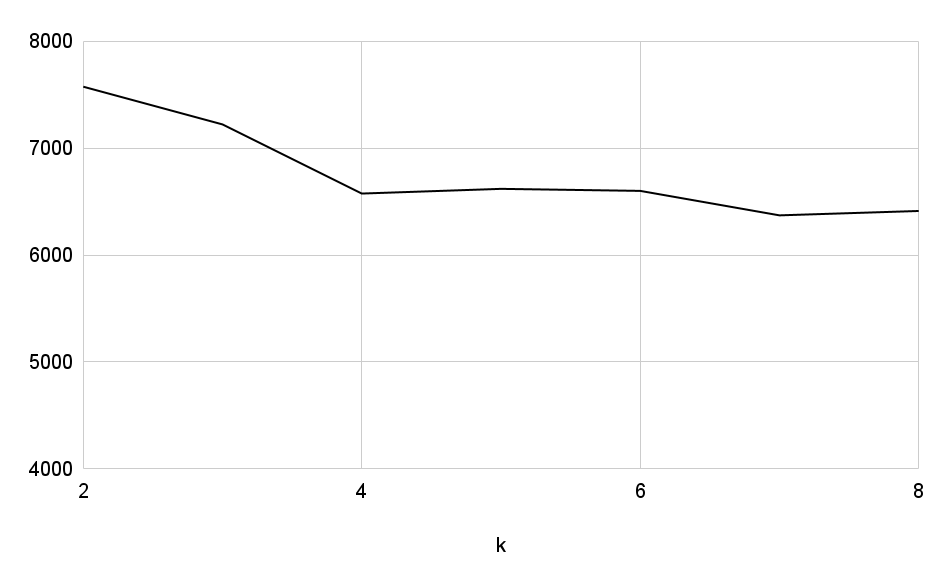
\includegraphics[width=0.7\linewidth]{img/chart.png}
\caption{$k$-means testing loss}
\end{figure}

The loss decreases dramatically then plateaus at $k = 4$. This indicates an optimal number of clusters of either 3 or 4. The clusters themselves are interesting and deserve some analysis. The paper titles in each cluster for $k = 3$ is listed in appendix A. A scan through the text samples in each cluster reveals some very interesting conclusions. Most notably, there is no clear split of text between different academic disciplines or branches of study. Each cluster contains texts from a wide variety of disciplines and the difference in distribution between each cluster in likely due to random chance.

This was puzzling, so I did a deeper dive. After manually reading the text within each cluster, it appears that text in the same cluster is written with a similar voice for audiences of similar academic sophistication. In appendix A, the clusters are labelled with the names \say{high school}, \say{undergrad}, and \say{graduate}, representing this distinction. I therefore conjectured that the distribution of POS transitions may be a good feature for identifying text with similar voice and lexical complexity. Since this conclusion comes from one person's subjective reading of a curated set of text, more work is necessary to come to solid conclusions. As a first start, I describe in section 3.3 a preliminary experiment that explores this conjecture.

\subsubsection{Markov Models}
I ran a classification task on the genres \textit{learned}, \textit{romance}, \textit{lore}, and \textit{mystery}, reserving 20\% of each genre as a testing set. The results with both the unigram and bigram models are summarized in figure 3.

\begin{figure}[ht!]
\begin{subfigure}[h]{\linewidth}
\centering
\begin{tabular}{|c|c|c|c|c|c|}
\hline
\textit{1-grams} & Learned & Romance & Lore & Mystery & Accuracy\\
\hline
Learned & 14 & 0 & 2 & 0 & 0.875\\
\hline
Romance & 0 & 4 & 0 & 1 & 0.800\\
\hline
Lore & 2 & 0 & 7 & 0 & 0.778\\
\hline
Mystery & 0 & 1 & 0 & 3 & 0.750\\
\hline
\end{tabular}
\subcaption{Classification results with unigram Markov model}
\end{subfigure}

\hfill
\begin{subfigure}[h]{\linewidth}
\centering
\begin{tabular}{|c|c|c|c|c|c|}
\hline
\textit{2-grams} & Learned & Romance & Lore & Mystery & Accuracy\\
\hline
Learned & 13 & 0 & 3 & 0 & 0.813\\
\hline
Romance & 2 & 2 & 0 & 1 & 0.400\\
\hline
Lore & 5 & 1 & 3 & 0 & 0.333\\
\hline
Mystery & 4 & 0 & 0 & 0 & 0.000\\
\hline
\end{tabular}
\subcaption{Classification results with bigram Markov model}
\end{subfigure}
\caption{Classification Results}
\end{figure}

The results for the unigram models are quite good. The model is not as very accurate at distinguishing between the two nonfiction (learned and lore) or fiction (romance and mystery) genres, but appears to have no trouble distinguishing nonfiction from fiction. This supports my hypothesis that word choice and writing style differs markedly between nonfiction and fiction genres.

The results for the bigram model are markedly less stellar. Although one might assume a more powerful model would result in more accurate classification, this does not appear to be the case for this experiment. I propose several explanations for the disparity between prediction and result.

Firstly, the state space is much larger so each matrix is much more sparse. Thus, each row in the matrix is trained on less data and is more likely to suffer from sampling error. In essence, we are training the bigram model on less data so it is less accurate than the unigram model.

Secondly, the likelihood estimation method cannot deal with zeroes in the matrix. In the case that the model has never been trained on a transition, it assigns likelihood 0 to that transition and thus to the text as a whole. Thus, any genre which has values for all of a text's transitions will achieve a higher likelihood, regardless of how similar the text actually is to the genre. This may explain why all of the predictions skew so heavily to \textit{learned}. Due to being trained on more physical text, it is more likely to contain some of the rarer transitions that other models have never seen.

There is unfortunately not a great fix for this problem. We may consider amending the likelihood estimation method to deal with zeroes in a complex way, but this would likely only be a stopgap for this specific corpus and model. Ultimately we simply need to train the model on more text.

\subsubsection{Non-fiction Genre Discrimination: A Case Study}
In section 3.1 I hypothesize that POS Markov models are useful in distinguishing genres with distinct voices. To test this hypothesis, I attempted to distinguish the \textit{learned} and \textit{news} genres with the unigram Markov model. Though both are nonfiction genres, news reportage has a very distinctive voice that, if I am correct, should allow the model to easily classify the two genres. Figure 4 summarizes my results using a testing set of 20\%.

\begin{figure}[ht!]
\centering
\begin{tabular}{|c|c|c|c|}
\hline
 & Learned & News & Accuracy\\
\hline
Learned & 16 & 0 & 1.000\\
\hline
News & 1 & 7 & 0.875\\
\hline
\end{tabular}
\caption{Learned vs News genres under unigram Markov model}
\end{figure}
The classification is very good, supporting our conjecture. More work is doubtless necessary to come to workable conclusions, but this is a start.

\subsection{Conclusion and Further Work}
This project explores a principled approach to genre discrimination. I drew upon work in computational linguistics to create a human-like approach to text classification. My model is highly explainable and performs decently against the state of the art. Markov transition models on bigrams appear to perform worse than models on unigrams but this is likely due to a lack of training data in our experiment. I suspect that more data will improve performance significantly. Unfortunately, due to time constraints for this project, I was unable to find and preprocess a corpus similar enough to the Brown corpus to augment our dataset.

I also conjecture that POS transition models are well-suited to capture voice and lexical complexity. A preliminary experiment supports this conclusion but future work should explore this connection further. In addition, this project explores temporal connection in a very limited sense. A Markov model \say{forgets} everything immediately after it passes into the past. Gains may be had by using a more sophisticated temporal model, such as a recurrent neural network, but care should be made to maintain explainability.


% -----------------------------------------------------------------------------
% -----------------------------Representation with Deep CCA--------------------
% -----------------------------------------------------------------------------

\section{Multi-View Representation Learning with Deep CCA}
\subsection{Introduction}
As our world becomes more and more saturated in technology, we have been able to gather data from multiple sensory perspectives. Something even as rudimentary as a parking sensor might simultaneously collect visual information and infrared distance measurements. A major point of study is to how we can relate different representational views of data to draw correlations between them. To use the parking example, we might want to find the distance to an object from a picture captured by the backup camera. My project aims to learn a common representation from the text and corresponding images of food recipes so we can use it for image to text and text to image retrieval. The commonly used model of \textit{canonical correlation analysis} (CCA)~\cite{HardoonSS04} gives satisfactory results for linear data but it does not fit well to non-linear data. Instead, I build on classic linear CCA with a non-linear deep CCA (with triplet loss) ~\cite{CCATripletLoss,GuerreroPP21} for image-text and text-image retrieval.

\subsection{Data and Methods}
\subsubsection{Dataset}
For my experiments, I used the Recipe1M dataset~\cite{Recipe1M}, containing over 1 million recipes with titles, instructions, ingredients, and corresponding pictures. However, since the dataset is quite large, I worked with a smaller subset containing around 400 thousand recipes and images. In addition, the dataset provided contains \textit{featurized} data, that is, data that has already been preprocessed to extract only the useful parts of each data value. For the text data, there are whole text embeddings that contain the title, ingredients, and instructions and single embeddings which contain either titles, ingredients, or instructions.

\subsubsection{Deep CCA Model}
To understand deep CCA, we first discuss conventional CCA. CCA is traditionally a dimensionality-reduction tool for paired data. If we have corresponding data in very high dimensions, we can \say{learn} a shared \textit{latent dimension} (typically much lower than the data provided) that preserves much of the correlation in the higher-dimensional spaces. Crucially, we are not learning the \textit{same} reduced space for both data views, only a transformation between them. We can extend CCA naturally to retrieval by using \textit{cosine similarity} on the data points. If we query a data point in one view, we can use the learned CCA transformation to project it into the other view, then find data points in the other view that are similar to that transformed query.

Deep CCA extends traditional CCA by attaching a deep neural net. The specifics of neural net architecture are not particularly interesting or illuminating, so are omitted here. The only thing to note is that instead of plugging the data directly into CCA, we run it through the neural net first. This allows us to learn nonlinear relationships in the data that are otherwise impossible to capture with vanilla CCA.

I traind the model using standard techniques for deep neural nets. In particular, I used a triplet loss function where the loss is measured as the difference in similarity between an \textit{anchor} image and two text representations, a \textit{positive} representative we know is similar to the image and a \textit{negative} representative we know is dissimilar. The goal of training is to maximize the correlation between the anchor and positive while minimizing the correlation between anchor and negative. Training is done iteratively using stochastic gradient descent, where the parameters of the model are tuned via backpropagation to minimize this loss with each new data point introduced.

%------------------------------------------------------------------------
\subsubsection{Evaluation}
To evaluate model performance, I used two standard metrics for retrieval tasks: \textit{median rank} (medR) and \textit{recall rate at top K} (R@k). Both of them are used by related tasks in ~\cite{Recipe1M} and ~\cite{xmrs} so can be considered standard academic benchmarks. We calculate the metrics by looking over a random sample of data points, typically 1 thousand or 10 thousand. Out of these random samples, we compute their ranks based on the results of cosine similarity and find the portion of pairs are selected in the top 1/5/10, corresponding to R@1, R@5 and R@10. We repeat this process 10 times and average the results.

%------------------------------------------------------------------------
\subsection{Results}

\subsubsection{Latent Dimension on CCA}
In my experiments, I chose different initial latent dimension from the range 10 to 1,000. The quantitative results are shown in table \ref{tab:cca-dim}. As expected, medR decreases with increased latent dimension, but plateaus after 100-200 dimensions. We see a similar trend in R@K, where recall increases quickly but plateaus after a while.

To find the optimal latent dimension that achieves medR 1, I ran some more fine-tuned experiments. For the dataset I used, the optimal dimension is in the range of 360 to 370 and is consistent for both text-to-image and image-to-text. A visualization of this is plotted in figure \ref{fig:fig1}.


\begin{figure*}
\begin{center}
  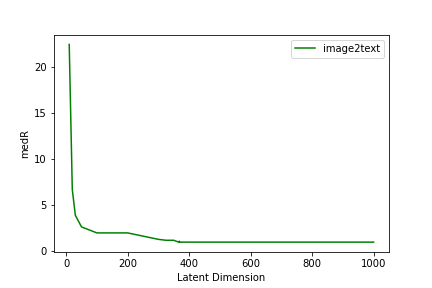
\includegraphics[width=0.45\linewidth]{img/image2text.png}
  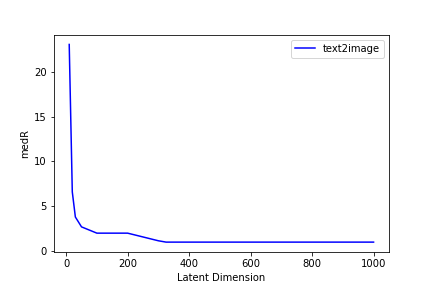
\includegraphics[width=0.45\linewidth]{img/text2image.png}
\end{center}
   \caption{Latent Dimension and medR}
\label{fig:fig1}
\end{figure*}


\begin{table*}[]
\begin{center}
\caption{Ablations studies on CCA dimension}
\label{tab:cca-dim}
\begin{tabular}{|l|llll|llll|}
\hline
         & \multicolumn{4}{c}{image2text} & \multicolumn{4}{|c|}{text2image} \\ \cline{2-9}
CCA Latent Dimension & medR   & R@1   & R@5   & R@10  & medR   & R@1   & R@5   & R@10  \\ \cline{1-9}
10   & 22.45  & 0.05  & 0.20  & 0.32  & 23.05  & 0.06  & 0.20  & 0.32  \\
20   & 6.7    & 0.17  & 0.45  & 0.61  & 6.6    & 0.17  & 0.46  & 0.61  \\
30   & 3.9    & 0.26  & 0.59  & 0.73  & 3.8    & 0.27  & 0.59  & 0.72  \\
50   & 2.65   & 0.34  & 0.69  & 0.80  & 2.7    & 0.35  & 0.67  & 0.79  \\
100  & 2.0    & 0.40  & 0.74  & 0.84  & 2.0    & 0.41  & 0.73  & 0.83  \\
200  & 2.0    & 0.47  & 0.78  & 0.85  & 2.0    & 0.48  & 0.77  & 0.85  \\
500  & 1.0    & 0.54  & 0.79  & 0.85  & 1.0    & 0.55  & 0.79  & 0.84  \\
1000 & 1.0    & 0.55  & 0.76  & 0.81  & 1.0    & 0.55  & 0.77  & 0.81  \\
\hline
\end{tabular}
\end{center}
\end{table*}

\subsubsection{Ablation on text elements}
In order to compare the impact of different text elements CCA on recall, I also conducted an ablation analysis on different combinations of text embeddings. The full results are shown in appendix B and are summarized here.

I found that the contribution of ingredients (\textit{ingr}) and instructions (\textit{instr}) were very similar and offer better performance than just titles (table \ref{tab:cca-element-500}). This is to be expected and served as a good sanity check. After all, ingredients and instructions provide much more information than titles so intuitively we expect them to perform better.

In addition, using two text embeddings was better than just one. But I found that pairing ingredients with another embedding yielded the best performance. In other words, ingredients contribute the most to final model performance than instructions or title.

Just for my curiosity, I also ran some experiments with latent dimension 100 and search space 1/10K. When latent dimensions are low, the combination of ingredients and instructions is the best on all metrics. So we can definitively say instructions contribute more information than titles for retrieval.

\subsection{Conclusion}
In this project, I explored deep CCA as a method of cross-representation learning. Although the project specification was outlined by the professor, the finer theoretical and implementation details had to be fleshed out through literature review and trial and error. The project directions simply said to \say{use deep CCA with triplet loss}; it was up to me to figure out how to theoretically build the model. For instance, CCA typically is trained on the entire dataset in one shot and deep models are trained iteratively using stochastic gradient descent, so I had to find a way to modify the standard CCA model to train with the neural net. In addition, my original model implementation trained incredibly slowly (10\% completion at 6 hours) so I had to research faster CCA implementations, ultimately settling on an iterative technique~\cite{Hotelling1992-jg} that improved model training time to under an hour.

Along the way, I learned a lot about the state-of-the-art in cross-representation learning. CCA methods are almost never used now, and the best current models almost exclusively use \textit{transformers}, a deep model that mimicks cognitive attention. It would be interesting to see how the model I developed compares to a modern transformer-based model. This may be a project I tackle some time in the future.

\section{Purpose}
When was first introduced to the concept of AI, it was couched in buzzwords and mystique. Billed as a panacea to solve all manner of problems, it seemed best to not ask too many questions and just trust the process. But curiosity got the better of me, and I peered deeper and deeper into the shrouded forest of knowledge.

I learned about decision trees; heuristic search; nonlinear regression; Laplacian mapping; hidden Markov models; deep, convolutional, and recurrent neural nets. As I learned more about something, the less impressed I was with it. At every step, I found myself thinking \say{wait\ldots that's it?} What had been billed as a mysterious black box descended from the heavens was nothing but math with extra steps. Thus began my disillusionment with the field of AI. \textit{If it's nothing but math anyways, I'll let the other people handle it}, I thought. I'll focus on more interesting theoretical problems instead. So I began to put less and less effort into my studies as I lost motivation to care about the nuances of learning rate scheduling, whatever that was.

For an academic, this kind of apathy is a death sentence, and I am fortunate to have discovered my disinterest early in my career. I wish I could say I've totally overcome this mental block, but I haven't. AI has certainly lost its luster the more I learn about it. But with a little soul-searching, I've come to think about it from a different perspective---it goes back to our discussion of artifice.

From the very beginning, people have developed algorithms to solve problems. AI is no exception. Think of Deep Blue, the first chess engine to beat world champion Garry Kasparov. At the end of the day, Deep Blue was just a big bruteforce decision tree that calculated all the possible moves up to a fixed depth. Is that intelligent? What about Magnus Carlsen, reigning world champion, whose theoretical knowledge allows him to analyze lines even deeper than Deep Blue. Is he intelligent? The answer I've come to is that it doesn't matter. Magnus is successful because of his ingenuity. When push comes to shove, his creativity over the board gives him an edge over his opponents. And AI are successful for the same reason---the human ingenuity it took to develop them. At the end of the day, it is all about our humanity. Our mental computing might be dwarfed by modern computers but human ingenuity is infinite. And as long as we are able tap into our ingenuity, there will always be room to grow.


\begin{appendices}
\section{3-cluster Results}
\begin{tabular}{|ll|}
\hline
\textbf{\say{High school} Cluster} & \\
\hline
Cornell H. Mayer & Radio. Emission of the Moon and Planets\\
\hline
B. J. D. Meeuse & The Story of Pollination\\
\hline
S. Idell Pyle et al. & Onsets, Completions \& Spans\\
\hline
Jacob Robbins et al. & The Thyroid-Stimulating Hormone\\
\hline
J. W. C. Hagstrom et. al. & Debilitating Muscular Weakness\\
\hline
E. Gellhorn & Prolegomena to a Theory of the Emotions\\
\hline
Max F. Millikan \& Donald L. Blackmer, editors & The Emerging Nations\\
\hline
Joyce O. Hertzler & American Social Institutions\\
\hline
Sister Claire M. Sawyer & Some Aspects of Fertility of a Tri-Racial Isolate\\
\hline
Dale L. Womble & Functional Marriage Course for the Already Married\\
\hline
Jesse W. Grimes \& Wesley Allinsmith & Compulsivity, Anxiety \& School Achievement\\
\hline
Ralph Bc Long & The Sentence \& Tts Parts\\
\hline
William O'Connor & Stocks, Wheat \& Pharaohs\\
\hline
Allan J. Braff \& Roger F. Miller & Wage-Price Policies Under Public Pressure\\
\hline
Wallace Mendelson & Justices Black \& Frankfurter\\
\hline
Irving Perluss & Agricultural Labor Disputes in California 1960\\
\hline
Edwin L. Bigelow \& Nancy H. Otis & Manchester, Vermont, A Pleasant Land\\
\hline
Jimmy Ernst & A Letter to Artists of the Soviet Union\\
\hline
I. B. M. Corporation & IBM 7070, Autocoder Reference Manual\\
\hline
Thomas D. McGrath & Submarine Defense\\
\hline
Nat'l Research Council & Directory of Continuing Numerical Data Projects\\
\hline
Harlan W. Nelson & Food Preservation by Ionizing Radiation\\
\hline
W. K. Asbeck & Forces in Coatings Removal Knife Cutting Method\\
\hline
Joel Frados, editor & Survey of Foamed Plastics\\
\hline
\end{tabular}
\begin{tabular}{|ll|}
\hline
Paul J. Dolon \& Wilfrid F. Niklas & Gain \& Resolution of Fiber Optic Intensifier\\
\hline
Rutherford Aris & The Optimal Design of Chemical Reactors\\
\hline
C. J. Savant Jr. \& R. C. Howard & Principles of Inertial Navigation\\
\hline
\end{tabular}
\\
\\
\noindent
\begin{tabular}{|ll|}
\hline
\textbf{\say{Undergrad} Cluster} &\\
\hline
J. F. Vedder & Micrometeorites\\
\hline
M. Yokayama et al & Chemical \& Serological Characteristics\\
\hline
Clifford H Pope & The Ciant Snakes\\
\hline
Kenneth Hoffman \& Ray Kunze & Linear Algebra\\
\hline
Howard J. Parad & Preventive Casework: Problems \& Implications\\
\hline
William H. Ittelson \& Samuel B. Kutash, editors & Perceptual Changes in Psychopathology\\
\hline
Harold Searles & Schizophrenic Communication\\
\hline
H.A. Cleason & Review of African Language Studies\\
\hline
Committee for Economic Development & Distressed Areas in a Growing Economy\\
\hline
James J. O'Leary & The outlook for Interest Rates in 1961\\
\hline
Albert Schreiber et al. & Defense Procurement \& Small Business\\
\hline
Irving L. Horowitz & Philosophy, Science \& the Sociology of Knowledge\\
\hline
Brand Blanshard & The Emotive Theory\\
\hline
Robert A. Futterman & The Future of Our Cities\\
\hline
Allyn Cox & Completing \& Restoring the Capitol Frescos\\
\hline
John H. Schaar & Escape from Authority, Perspectives of Erich Fromm\\
\hline
Katherine G. McDonald & Figures of Rebellion\\
\hline
Samuel Hynes & The Pattern of Hardy's Poetry\\
\hline
Kenneth Rexroth & Disengagament: The Art of the Beat Generation\\
\hline
\end{tabular}

\noindent
\begin{tabular}{|ll|}
\hline
\textbf{\say{Graduate} Cluster} & \\
\hline
R. C. Binder et al. 1961 & Heat Transfer \& Fluid Mechanics Institute\\
\hline
Harry H. Hull & Normal Forces \& Their Thermodynamic Significance\\
\hline
James A. Ibers et al. & Proton Magnetic Resonance Study\\
\hline
John R. Van Wazer, ed. & Phosphorus and Its Compounds\\
\hline
Francis J. Johnston \& John E. Willard & Exchange Reaction Between Cl2 and CCl4\\
\hline
LeRoy Fothergill & Biological Warfare\\
\hline
Richard F McLaughlin et al. & A Study of the Subgross Pulmonary Anatomy\\
\hline
A. N. Nagaraj \& L. M. Black & Localization of Wound-Tumor Virus Antigen\\
\hline
Frederick Mosteller et al. & Probability with Statistical Applications\\
\hline
R. P. Jerrard & Inscribed Squares in Plane Curves\\
\hline
C. R. Wylie, Jr. & Line Involutions in S3\\
\hline
Frank Lorimer & Demographic Information on Tropical Africa\\
\hline
Raymond J. Corsini & Roleplaying in Business \& Industry\\
\hline
Hugh Kelly \& Ted Ziehe & Glossary Lookup Made Easy\\
\hline
A. T. Kroeber & Semantic Contribution of Lexicostatistics\\
\hline
D. F. Fleming & The Cold War \& Its Origins\\
\hline
Douglas Ashford & Elections' in Morocco: Progress or Confusion\\
\hline
Morton A. Kaplan \& Nicholas Katzenbach & The Political Foundation of Internationa1 Law\\
\hline
J. Mitchell Reese, Jr, & Reorganization Transfers\\
\hline
William S. Ragan & Teaching America's Children.\\
\hline
Paul Cooke & Desegregated Education in the Middle-South Region\\
\hline
Robert J. Havighurst & Social-Class Influences on American Education\\
\hline
James C. Bonbright & Principles of Public Utility Rates\\
\hline
William S. Haymond & Is Distance an Original Factor in Vision?\\
\hline
Chester G. Starr & The Origins of Greek Civilization 1100-650 B. C\\
\hline
Jim B. Pearson & The Maxwell Land Grant\\
\hline
\end{tabular}
\begin{tabular}{|ll|}
\hline
J. H. Hexter & Thomas More: on the Margins of Modernity\\
\hline
John M, Ray & Rhode Island's Reactions to John Brown's Raid\\
\hline
Clement Greenberg & Collage\\
\hline
William Whallon & The Diction of Beowulf\\
\hline
Charles R. Forker & The Language of Hands in Great Expectations\\
\hline
Ross E. McKinney \& Howard Edde & Aerated Lagoon for Suburban Sewage Disposal\\
\hline
Mellon Institute & Annual Report; 1960, Independent Research\\
\hline
William D. Appel, editor & 1961 Technical Manual of American Ass'n of Textile\\
 & Chemists \& Colorists\\ % page break
\hline
\end{tabular}

\section{Ablation studies on text elements}
\begin{table*}[h]
\begin{center}
\caption{Ablations studies on different text elements with 500 latent dimensions}
\label{tab:cca-element-500}
\begin{tabular}{|l|llll|llll|llll|llll|}
\hline
\toprule
& \multicolumn{4}{c|}{image2text} & \multicolumn{4}{|c|}{text2image}  \\ \cline{2-9}
Text elements & medR   & R@1   & R@5   & R@10  & medR   & R@1   & R@5   & R@10   \\ \cline{1-9}
\midrule
All & 1.0 & 0.54 & 0.79 & 0.84 & 1.0 & 0.55 & 0.79 & 0.84 \\
Ingr & 3.0 & 0.35 & 0.59 & 0.67 & 3.0 & 0.36 & 0.60 & 0.67 \\
Instr & 3.0 & 0.35 & 0.60 & 0.68 & 3.0 & 0.36 & 0.61 & 0.68 \\
Titles & 10.2 & 0.22 & 0.43 & 0.50 & 10.5 & 0.22 & 0.43 & 0.50 \\
Ingr+instr & 2.0 & 0.44 & 0.71 & 0.77 & 2.0 & 0.46 & 0.72 & 0.78 \\
Ingr+title & 2.0 & 0.39 & 0.65 & 0.72 & 2.0 & 0.39 & 0.65 & 0.72 \\
Instr+title & 2.7 & 0.37 & 0.63 & 0.71 & 2.2 & 0.38 & 0.64 & 0.71 \\
\bottomrule
\hline
\end{tabular}
\end{center}
\end{table*}

\begin{table*}[h]
\caption{Ablations studies on different text elements with 100 latent dimensions and 1K/10K search size}
\label{tab:diff-elements}
\centering
\begin{tabular}{|l|llll|llll|}
\hline
\toprule
& \multicolumn{8}{c|}{1K}\\ \cline{2-9}
& \multicolumn{4}{c|}{image2text} & \multicolumn{4}{|c|}{text2image}\\ \cline{2-9}
& medR   & R@1   & R@5   & R@10  & medR   & R@1   & R@5   & R@10 \\ \cline{1-9}
\midrule
All & 2.0 & 0.40 & 0.74 & 0.84 & 2.0 & 0.41 & 0.73 & 0.83 \\
Ingr & 3.9 & 0.27 & 0.57 & 0.70 & 3.9 & 0.28 & 0.58 & 0.70 \\
Instr & 4.0 & 0.27 & 0.58 & 0.71 & 3.9 & 0.28 & 0.59 & 0.72 \\
Titles & 7.85 & 0.16 & 0.43 & 0.56 & 8.35 & 0.16 & 0.42 & 0.54 \\
Ingr+instr & 2.6 & 0.34 & 0.68 & 0.80 & 2.0 & 0.37 & 0.70 & 0.80 \\
Ingr+title & 3.0 & 0.32 & 0.65 & 0.76 & 3.0 & 0.32 & 0.65 & 0.76 \\
Instr+title & 3.1 & 0.28 & 0.62 & 0.75 & 3.0 & 0.30 & 0.63 & 0.76 \\
\bottomrule
\hline
\end{tabular}
\end{table*}

\begin{table*}[h]
\centering
\begin{tabular}{|l|llll|llll|}
\hline
\toprule
& \multicolumn{8}{c|}{10K}\\ \cline{2-9}
& \multicolumn{4}{c|}{image2text} & \multicolumn{4}{|c|}{text2image}\\ \cline{2-9}
& medR   & R@1   & R@5   & R@10  & medR   & R@1   & R@5   & R@10 \\ \cline{1-9}
\midrule
All & 12.0 & 0.14 & 0.35 & 0.47 & 12.0 & 0.15 & 0.36 & 0.48 \\
Ingr & 28.4 & 0.08 & 0.22 & 0.32 & 27.5 & 0.09 & 0.24 & 0.33 \\
Instr & 29.8 & 0.07 & 0.21 & 0.31 & 28.7 & 0.08 & 0.22 & 0.32 \\
Titles & 67.7 & 0.03 & 0.12 & 0.19 & 71.6 & 0.03 & 0.11 & 0.19 \\
Ingr+instr & 17.1 & 0.11 & 0.29 & 0.40 & 15.0 & 0.13 & 0.32 & 0.43 \\
Ingr+title & 20.6 & 0.09 & 0.26 & 0.37 & 19.9 & 0.10 & 0.27 & 0.38 \\
Instr+title & 24.9 & 0.08 & 0.23 & 0.33 & 23.8 & 0.08 & 0.24 & 0.34 \\
\bottomrule
\hline
\end{tabular}
\end{table*}

\end{appendices}

\newpage
\bibliography{report}

\end{document}

% List of tex snippets:
%   - tex-header (this)
%   - R      --> \mathbb{R}
%   - Z      --> \mathbb{Z}
%   - B      --> \mathcal{B}
%   - E      --> \mathbb{E}
%   - M      --> \mathcal{M}
%   - m      --> \mathfrak{m}({#1})
%   - normlp --> \norm{{#1}}_{L^{{#2}}}
%   - dd     --> \;\mathrm{d}{#1}
